\begin{figure*}[t]
  \centering
  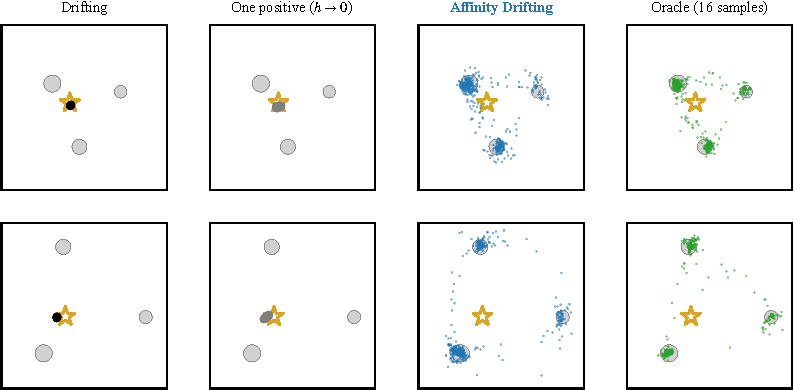
\includegraphics[width=\linewidth]{generated/figures/fig_teaser}
  \caption{\textbf{Mean collapse with one positive per condition.} Samples (512 per panel) from generators trained on a
  2-D toy where each training condition $c$ has exactly one sample, on two held-out conditions. Grey: true
  $p(x\mid c)$, a three-mode mixture; hollow $\star$: the conditional mean $\mathbb E[x\mid c]$. The original Drifting
  objective and the single-positive objective put every sample at the conditional mean, between the modes; an oracle
  given many true samples per condition covers the modes. \affd uses only the single positives, borrowed across similar
  conditions, and recovers the modes. Held-out conditions, seed 0 of five.}
  \label{fig:teaser}
\end{figure*}

\section{Introduction}
\label{sec:intro}

One-step generators trained by \emph{drifting}~\cite{deng2026drifting} evolve the pushforward of a noise distribution
during training rather than at sampling time: each generated sample is attracted toward data and repelled from the
other samples, and the generator regresses onto its own drifted outputs. With class labels, every class has many
images and the attraction is a proper mean-shift toward the class distribution.

Text conditioning breaks that assumption. A caption typically describes one image, so the positive set of a condition
has size one. Then the normalised attraction weight is one and the attraction no longer depends on where the sample
is: it is $L_2$ regression onto the single positive (Lemma~\ref{lem:regression}). A generator with finite resolution in
$c$ averages the positives of conditions it cannot tell apart and outputs their mean --- a blurred blob between modes
(\cref{fig:teaser}).

We ask whether \emph{borrowing} positives from semantically close conditions restores a distribution, and why. \affd
weighs every positive $y_i$ by a caption affinity $w_i(c)$ and keeps the $x$-dependent kernel of drifting, so the
attraction becomes a mean-shift toward a mixture rather than a pull toward an average. The claim is mechanistic: the
gain should come from the $x$-dependent mode assignment, not merely from having more targets. We therefore test it
with controls that remove each alternative explanation in turn --- averaging targets without $x$-dependence (K1),
random instead of semantic neighbours (K2), noise-smoothed single targets (K3) --- against an oracle with true samples
(K4) and the original Drifting objective as a baseline.

\paragraph{Contributions.} (i) The single-positive degeneracy of drifting and its consequence, mean collapse under
limited conditional capacity. (ii) \affd, with a fixed-point analysis for Gaussian kernels. (iii) A pre-registered,
single-factor experimental protocol, run bottom-up from particles to neural toys; this draft reports what is
finished and marks the rest as pending.
